\documentclass{ctexart}

\usepackage{ctex}
\usepackage{subfigure}
\usepackage{CJK}
\usepackage{siunitx}
\usepackage{amsmath}
\usepackage{amssymb}
\usepackage{graphicx}
\usepackage{cite}
\usepackage{multirow}
\usepackage{float}
\usepackage{xltxtra}
\usepackage[a4paper,left=1.25in,right=1.25in,top=1in,bottom=1in]{geometry}
%标题, 作者

\title{Julia Set 的生成}

\author{作者姓名: 唐浩 \\ 专业和学号: 信息与计算科学 3200102118}

\begin{document}

\maketitle

\renewcommand{\abstractname}{摘要} %摘要
\bibliographystyle{plain}

\begin{abstract}

  本文就 Julia Set 的生成进行探索,简要介绍一下 Julia Set 的起始,数学推导,并附上一定的图片解释。通过计算机,我们可以进行相对于人脑来说较麻烦的计算,通过计算机进行迭代,我们可以简单重现 Julia Set 的生成过程。并探讨 Julia Set 与 Mandelbrot Set 之间的关系
  
\textbf{关键字:Julia Set 迭代 Mandelbrot Set 图形生成{} 比较}

\end{abstract}

\section{引言} %引言
朱利亚集合(又译为茹利亚集合,英语:{\bf Julia se})是一个在复平面上形成分形的点的集合。以法国数学家加斯顿·朱利亚(Gaston Julia)的名字命名。
\begin{figure}[H]
\centering
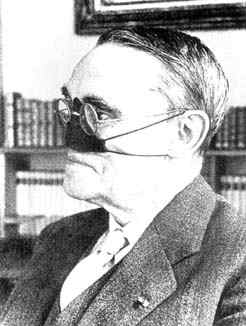
\includegraphics[scale=0.3]{Julia.jpeg}
\end{figure}
它是一个几何图形,其中的点均出自迭代公式:{\bf $Z_{n+1} = Z_n^2 + C$},取定一个常数C, 对于复平面上的每一点 z,若$Z_n$收敛,则 z 在集合中。对于所有的 z 组成的集合,便称为{\bf Julia Set}。本文主要介绍如何生成 Julia Set,并简单叙述其与 Mandelbrot Set 之间的关系。


%数学理论, 算法, 数值算例, 结论
\section{数学理论}
\subsection{迭代}

首先,我们来介绍一下什么是迭代。迭代是重复反馈过程的活动,其目的通常是为了逼近所需目标或结果。每一次对过程的重复称为一次“迭代”,而每一次迭代得到的结果会作为下一次迭代的初始值。就 Julia Set 而言,被迭代的是一些最简单的函数,其形如 $f(x) = x^2 + C$(C 为常量)。

对于每一个 z,若根据迭代规则: $Z_{n+1} = Z_n^2 + C$ 生成的序列$\{x_0, x_1,\dots\} \rightarrow \infty$ ,则Z的轨迹无界,则 $z \notin$  Julia Set,若序列有界,则 $z \in$ Julia Set 。

\subsection{逃逸时间算法}
\subsubsection{逃逸法则}

对于一个复数 $z_n = x_n + y_ni$, 模 $|z_n| = \sqrt{x_n^2 + y_n^2}$ 。定义:

如果对于一个复数序列 $\{z_1, z_2, \dots, z_n\}$ 有 $|z_j| > max(2,|C|)$ 则序列将逃逸到无穷大。

\subsubsection{逃逸时间算法}

对于每个复参数平面上的点C,我们生成一个序列Z,根据逃逸准则,我们规定R为逃逸半径,在 $\{z_1, \dots z_n\}$ 里,如果 $|z_j| < R$ ,判断有界(但其实也有可能这个序列是无界的),反之,这个序列无界。故需要确定以下参数:

1、复平面范围 $C = \{c = x + yi: x_1 \le x \le x_2, y_1 \le y \le y_2 \}$
  
2、分辨率gridSize

3、逃逸半径 $R = max(2, |C|)$

4、逃逸时间 N = 最大迭代次数

\section{算法}

\section{数值算例}

迭代次数取 N = 100,选取不同的常数 C, 将会得到不同的 Julia Set,以下我们简要选取几个常数 C 的值,通过计算机生成的bmp图像来观察不同的 C 所产生的 Julia Set:
当我们将 C 设置成(0,0),将会得到一个圆,由于图像的对称性,在此,统一将 C 取为(-x,y)的形式。
\begin{figure}[H]
\centering
\subfigure[C = (0,0)]
    {
        \centering
        \includegraphics[width=0.45\textwidth]{test0.bmp}
    }
\subfigure[C = (-0.5,0.5)]
    {
        \centering
        \includegraphics[width=0.45\textwidth]{test7.bmp}
    }
\end{figure}

\begin{figure}[H]
\centering
\subfigure[C = (-0.1,0.7)]
    {
        \centering
        \includegraphics[width=0.45\textwidth]{test8.bmp}
    }
\subfigure[C = (-1,0.2)]
    {
      \centering
      \includegraphics[width=0.45\textwidth]{test9.bmp}
    }
\end{figure}

如果我们将原点偏移,还可以得到一个具体部位的放大图,这里就不做举例了,感兴趣的读者可以自己修改参数,查看结果。

\section{分析}

让我们先生成一个 Mandelbrot Set 的图,取 N = 100,其生成的图如下所示:
\begin{figure}[H]
  \centering
  \includegraphics[scale=0.3]{test3.bmp}
  \caption{This is a Mandelbrot Set picture}
\end{figure}
注意到,图中的每个点对应于一个filled Julia Set,其中黑点是路径连通的 Julia Set,白点是不连通的 Julia Set。选取 Mandelbrot Set 中的对应黑点,便可得到上面生成的 Julia Set 图。

与我们看到的其他分形不同,Mandelbrot Set 的结构不是自相似的。相反,它在不同的地方有完全不同的局部结构。新的结构在每一个尺度上都被揭示出来,而这种模式似乎并不重复。同样的事情几乎会发生在 Mandelbrot Set 中的任何一点上,在每一点上都会显示出不同的结构。

Mandelbrot Set 与 Julia Set 都是由迭代关系: $z_{n+1} = z_n + C$ 所产生的点集,只不过两者一个由 z 产生,一个由 C 产生,在计算机上表现的不同便是一个遍历 z ,一个遍历 C 。

\section{结论}

Julia Set 和 Mandelbrot Set 的图形表示可以让我们认识到纯粹的数学之美,与之相关的分形几何学则是无处不在的,不得不感叹数学的力量。由于分形几何学知识的匮乏,本文只能给出Julia Set的定义,并以最容易理解的方式绘制出该集合。这里使用的语言是C++。 \cite{王伊蕾2015LaTeX}

\bibliographystyle{plain}
\bibliography{ckwx.bib}

\end{document}
